\documentclass[12pt]{report}
\usepackage[style=ieee]{biblatex}
\addbibresource{references.bib}
\usepackage{enumitem}
\setlist[enumerate]{nosep}
\usepackage{etoolbox}
\usepackage{fancyhdr}
\usepackage{float}
\usepackage{fontspec}
\usepackage[letterpaper,hmargin={47.5mm,17.5mm},top=64.0mm,bottom=25.4mm]{geometry}
\usepackage{indentfirst}
\usepackage{microtype}
\usepackage{multirow}
\usepackage{setspace}
\usepackage{tabularx}
\usepackage[explicit]{titlesec}
\usepackage{tocbibind}
\usepackage{wallpaper}

\newcommand{\authora}{
    Melba Dominique B. Castorico %
}
\newcommand{\authorb}{
    Basil Eric Rabi %
}
\newcommand{\authorc}{
    Herald Joy Dela Cruz %
}
\newcommand{\eg}{\emph{e.g.}}
\newcommand{\hypothesis}[3]{
\noindent \textbf{Research Question:}
\par#1
\begin{quotation}
    \noindent \textbf{Null Hypothesis ($H_o$)}:
    \par#2

    \noindent \textbf{Alternative Hypothesis ($H_a$)}:
    \par#3
\end{quotation}
}


\newcommand{\thetitle}{LOMOPTIM: An Implementation of Lerchs-Grossman Algorithm for Open Pit Mines with Sub-Optimal Conditions}

\usepackage[hidelinks]{hyperref}
\hypersetup{
    pdfborder  = {0 0 0},
    pdfinfo    = {
        Title    = {\thetitle},
        Subject  = {Mine Economics},
        Author   = {\authora and \authorb and \authorc},
        Keywords = {Optimization, Mining, Mine Economics, Strategic Mine Planning}
    }
}

\addtolength{\headwidth}{15pt}
\doublespacing
\renewcommand{\contentsname}{TABLE OF CONTENTS}
\renewcommand{\headrulewidth}{0pt}
\setmainfont[Mapping=tex-text-ms]{Times New Roman}
\setlength{\headheight}{15pt}
\setlength{\parindent}{12.7mm}
\setcounter{secnumdepth}{3}
\titleformat{\chapter}[block]{\bfseries\centering}{}{0em}{#1}
\titlespacing{\chapter}{0pt}{-30pt}{0pt}
\titlespacing{\section}{0pt}{0pt}{0pt}
\titlespacing{\subsection}{0pt}{0pt}{0pt}
\titlespacing{\subsubsection}{0pt}{0pt}{0pt}

\begin{document}

\ULCornerWallPaper{1}{spus.pdf}
\pagenumbering{roman}
\addcontentsline{toc}{chapter}{TITLE PAGE}
\thispagestyle{empty}

\begin{center}

\textbf{\MakeUppercase{\thetitle}}

\vspace{1.5cm}
A Research Concept Paper Presented to \\
The College of Engineering \\
St. Paul University Surigao

\vfill

In Partial Fulfillment of the Requirements for the Course \\
THESIS 1

\vspace{1cm}
By:

\vspace{1cm}
\textbf{\authora} \\

\vspace{1cm}
November 2023

\end{center}

\fancypagestyle{plain}{
    \fancyhead{}
    \fancyfoot{}
    \fancyhead[R]{\thepage}
}

\pagestyle{fancy}
\fancyhead{}
\fancyfoot{}
\fancyhead[R]{\thepage}

\tableofcontents

\titleformat{\chapter}[block]{\bfseries\centering}{CHAPTER \thechapter\\#1}{0em}{}
\titleformat{\section}[block]{\bfseries\centering}{\MakeUppercase{#1}}{0em}{}
\titleformat{\subsection}[block]{\bfseries}{#1}{0em}{}
\titleformat{\subsubsection}[block]{}{\emph{#1}}{0em}{}

\chapter{THE PROBLEM AND ITS BACKGROUND}

\pagenumbering{arabic}

\section{Introduction}

\subsection{Mineral Reserves and Optimized Strategic Plans for Surface Mines}

\subsubsection{Optimized Economics}

\subsubsection{Good Governance and Environmental Compliance}

\subsection{Challenges of Using Presently Available Tools for Strategic Mine Planning}

% Whittle and other alternatives

\subsubsection{Open Area Restriction}

\subsubsection{Minimum Throughput Requirements for Specific Products}

\subsection{Auditability}

\section{Conceptual Framework of the Study}

\section{Statement of the Problem}

\begin{enumerate}
    \item How is the system developed in relation to
            \begin{enumerate}
                \item Software stack selection
                \item Current tools used by the company
                \item End-user's requirement and feedback
            \end{enumerate}
    \item How efficient is the researcher's system terms of
        \begin{enumerate}
            \item Processing time in achieving the highest net present value
            \item Achieving the throughput requirement per product
            \item Achieving the yearly slices which complies to the environmental requirements
        \end{enumerate}
    \item What is the evaluation of the system by the experts and users in terms of
        \begin{enumerate}
            \item Efficiency
            \item User's experience
        \end{enumerate}
\end{enumerate}

\section{Hypothesis}

\hypothesis{
Does the researcher's system meet the technical expert's standards in terms of the system's efficiency and user's experience?
}{
The researcher's system did not meet the technical expert's standards based on the identified factors.
}{
The researcher's system meets the technical expert's standards based on the identified factors.
}

\hypothesis{
Are there any technical limitations that might hinder the system's adoption?
}{
There are technical limitations that might hinder the system's adoption.
}{
There are no technical limitations that might hinder the system's adoption.
}

\hypothesis{
Does the researcher's system address the identified challenges and problems?
}{
The researcher's system does not address the identified challenges and problems.
}{
The researcher's system addresses the identified challenges and problems.
}

\section{Significance of the Study}

\section{Scope and Limitation of the Study}

\chapter{REVIEW OF RELATED LITERATURE}

\chapter{METHODS}

\section{Research Design}

\section{Participants}

\section{Methodology}

\subsection{Formulation of Requirements}

The functionalities and the features of the data collection system will be identified first.
As the research progresses, the functionalities will be illustrated as use-case diagrams which are analogous to the design requirements \cite{UseCase}.
The formulation of requirements will depend upon the existing process and systems implemented by the host company.
The formulation of requirements is a way to identify the gaps in the company's process' efficiency that can be addressed by researcher's propose system.

\subsection{System Design}

\subsubsection{Use Case}

\subsubsection{File Structures}

\subsubsection{Data Structures}

\subsubsection{Algorithm}

\subsection{Source Code Writing}

\subsection{System Testing}

\section{Instruments}

On the software side of the development, free and open source tools will be used.

A similar method of evaluation will be used based on the ER Mine Tracer research design.
The researchers of the said study used survey to qualitatively evaluate ER Mine Tracer's functionality and efficiency.
In this study, the researchers will also employ surveys to gather qualitative data on the users' experience and opinion regarding the researcher's data collection and processing system \cite{ERMineTracer}.

Spreadsheet applications such Microsoft Excel or LibreOffice Calc will be used for data encoding and inspection while R version 4.3 \cite{R} will be used for data manipulation and analysis.

\section{Data Gathering Procedure}

\subsection{Quantitative Data}

The efficiency and effectiveness of LOMOPTIM will be evaluated in terms of compliance with the input restrictions and processing time.

\subsection{Qualitative Data}

A Likert 4-point scales for "Agreement" parameter with 0.25 point increment will be basis of point system of the survey questionnaire.
For each parameter, the verbal response and qualitative description provided by the system validators are used to generate the scale.
Depending on the name of the performance exam, the first scale, or maximum, ranges from 3.25 to 4.00 with a parameter of 4 and a vocal response of "strongly agree".
The second scale has a range of 2.5–3.25, a parameter of 3, an agree verbal response, and a qualitative description based on the name of the performance test.
The third scale has a parameter of 2, a verbal response of "disagree," and a qualitative description based on the name of the performance test.
Its range is 1.75-2.50.

The final scale has a range of 1.00 to 1.75, a parameter of 1, a verbal response of "strongly disagree," and a qualitative description based on the topic of the performance test \cite{Likert}.

\section{Data Analysis}

Descriptive statistics will be computed using quantitative data coming from SAFER during its testing.
The performance of LOMOPTIM will be compared to Whittle which is the existing system used by TMC.
The researchers will be using R version 4.3 \cite{R} to analyze the quantitative data.

Questionnaire surveys with qualitative information will be distributed to Strategic Mine Planners, IT Experts, Computer Engineers and other experts on this topic in order to collect data that are qualitative in nature.

The result of the surveys and the collected quantitative data will be used by the researchers to determine if LOMOPTIM meets the user's requirements, meets the standard's of the technical experts, and does not have any technical limitations that might hinder its adoption.

\section{Ethical Considerations}

The data collected in this study shall be subject to the stipulations of the Republic Act 10173 or the Data Privacy Act of 2012.
All the data gathering procedures shall be approved by the management of the host company, and shall be shared to them should they ask for it.
Should there be instances where sensitive data may need to be included in publications, the company's approval shall be acquired beforehand.


\titleformat{\chapter}[block]{\bfseries\centering}{}{0em}{#1}
\printbibliography[
    title = {REFERENCES},
    heading = bibintoc
]

\newgeometry{hmargin={47.5mm,20mm},top=64.0mm,bottom=25.4mm}
\setlength{\parindent}{0mm}

\begin{spacing}{1.55}

\chapter*{CURRICULUM VITAE}
\addcontentsline{toc}{chapter}{CURRICULUM VITAE}

\begin{tabularx}{\linewidth}{@{}lXr}
    \MakeUppercase{\authora} && \multirow{3}{*}{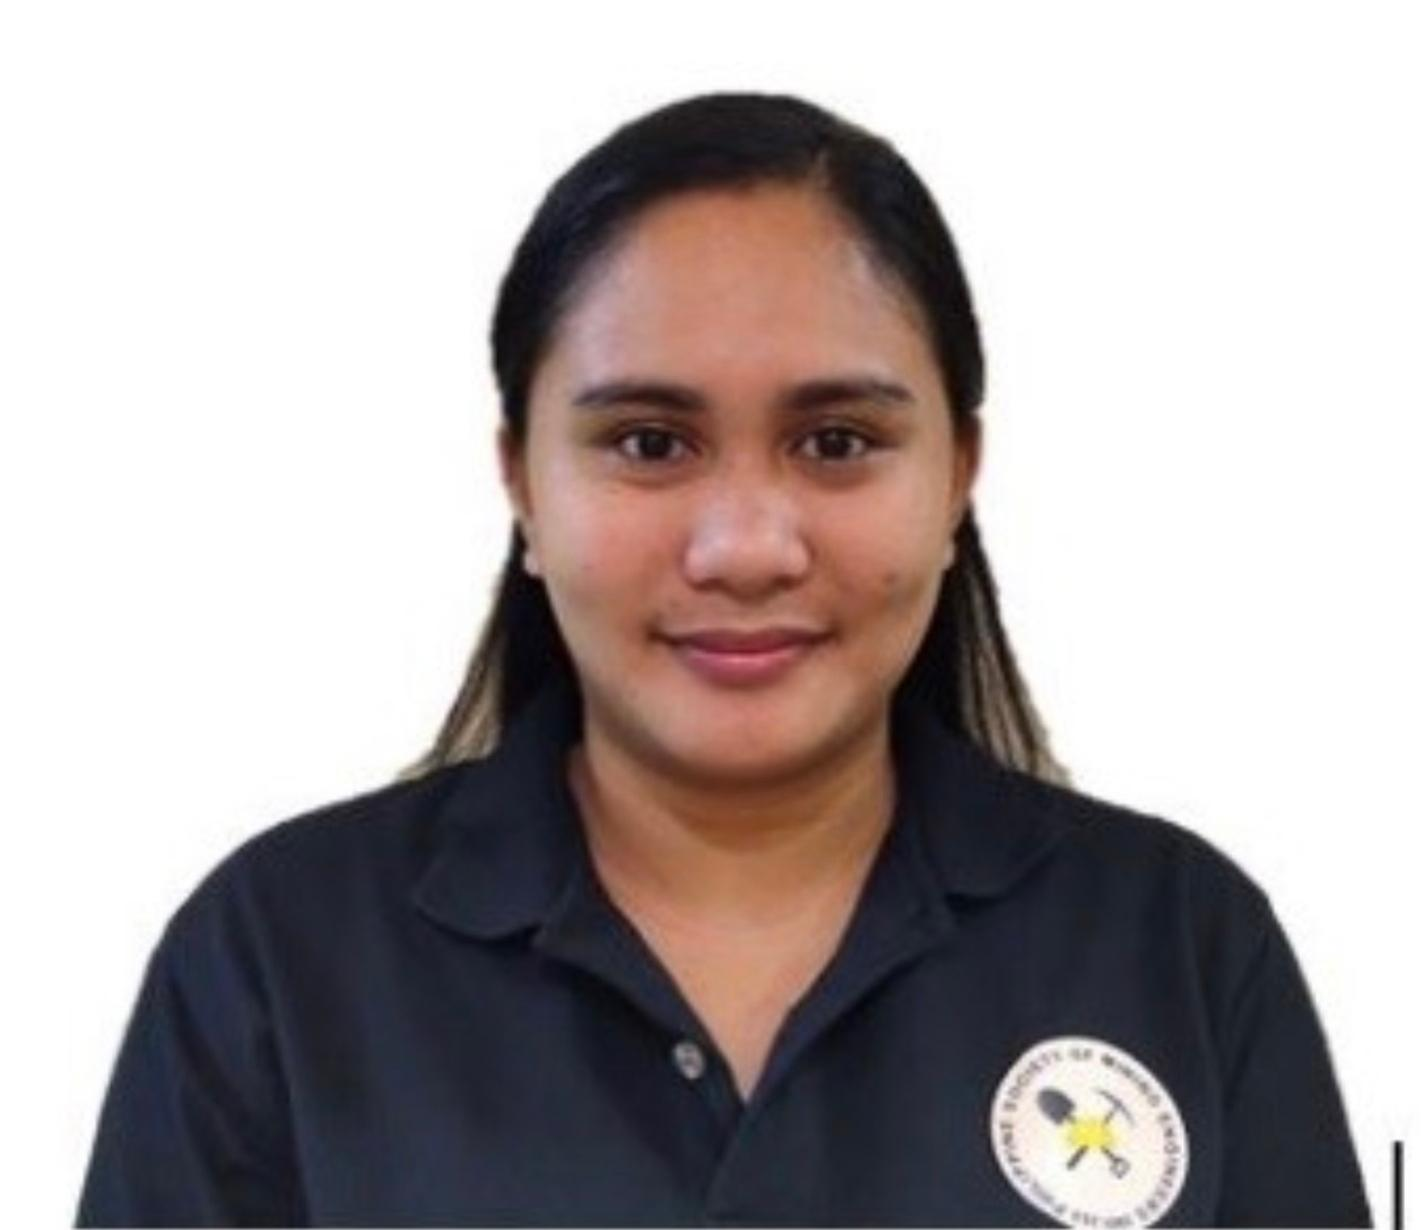
\includegraphics[width=1in]{img/burdeos}} \\ %TODO: Picture
    Insert address: Agusan del Norte && \\
    melba.dominque@gmail.com && \\
\end{tabularx}

\vspace{20pt}

\textbf{PERSONAL INFORMATION}

\vspace{-10pt}
\hrulefill

\begin{tabular}{@{}l@{ : }l}
    DATE OF BIRTH & June 1, 1992 \\
    PLACE OF BIRTH & TODO \\
    AGE & 31 \\
    GENDER & Female \\
    NATIONALITY & Filipino \\
    RELIGION & TODO \\
    CIVIL STATUS & Married \\
    FATHER'S NAME & TODO \\
    MOTHER'S NAME & TODO \\
\end{tabular}

\vspace{20pt}

\textbf{EDUCATIONAL BACKGROUND}

\vspace{-10pt}
\hrulefill

\begin{tabular}{@{}l@{ : }l}
    COLLEGE & Saint Paul University Surigao \\
    & Corner Rizal and San Nicolas Streets, Surigao City \\
    HIGH SCHOOL & TODO: High school name \\
    & TODO: High school address \\
    ELEMENTARY & TODO: Elementary school name \\
    & TODO: Elementary school address \\
\end{tabular}

\end{spacing}
\end{document}
